
\chapter{Introduction}

\vspace{3mm}
% \noindent\rule{17cm}{0.2pt}
\fbox {
    \parbox{\linewidth}{
      \begin{itemize}
        \item Motivation
        \item Aims
        \item Thesis outline
        \item Contributions to knowledge
      \end{itemize}
    }
}
\vspace{3mm}


\section{Motivation}

% cancer is bad
In an article titled "Is the world making progress against cancer?" \citep{Roser2015-qb}, the authors provide an overview of humanity's progress in combating the disease. Since cancer is typically a disease associated with ageing, the consequence of a longer-living global population is that more people are now affected by cancer; see overall cancer deaths in \cref{fig:cancer_death}. With the help of technological and biological progress made in the past decades, the welfare of the global population has improved, which is reflected in the standardised cancer death rates from 1990 to 2017, dropping by approximately 17\%. However, cancer remains a terrible disease, affecting the lives of too many patients and their families across the world.

% Bladder cancer
According to Cancer Research UK \citep{Cancer_Research_UK2015-cf}, bladder cancer is the 10th leading cause of cancer death, accounting for 3\% of all cancer-related deaths in the UK, with 56\% of cases occurring in people older than 75. Almost half (52.6\%) of those diagnosed with bladder cancer survive for more than five years, and 46.4\% survive for more than ten years.

% Introduce the MIBC
There are two major types of bladder cancer: \acrfull{nmibc} and \acrfull{mibc}. The former has a 5-year survival rate of around 90\% % but a high recurrence rate, impacting the quality of life. At the same time, the latter is more aggressive, with a higher chance of becoming metastatic and a worse 5-year survival rate of approximately 50\%. This project focuses on studying \acrlong{mibc}.

% Limitations with MIBC classifications
The current MIBC classifications \citep{Kamoun2020-tj,Robertson2017-mg,Marzouka2018-ge} were derived solely from tumour gene expression data. While some clinical trials \citep{Griffin2024-zr} are underway, these subgroups have yet to improve clinical outcomes significantly. The complex molecular characteristics of MIBC necessitate the development of subtypes based on multi-omics data integration.

% What we're doing
Therefore, the motivation of this project is to address the limitations of current MIBC stratification by developing a new integrative network approach to stratify \acrlong{mibc} in a way that is translatable to the clinic.


\begin{figure}[!htb]
    \centering
    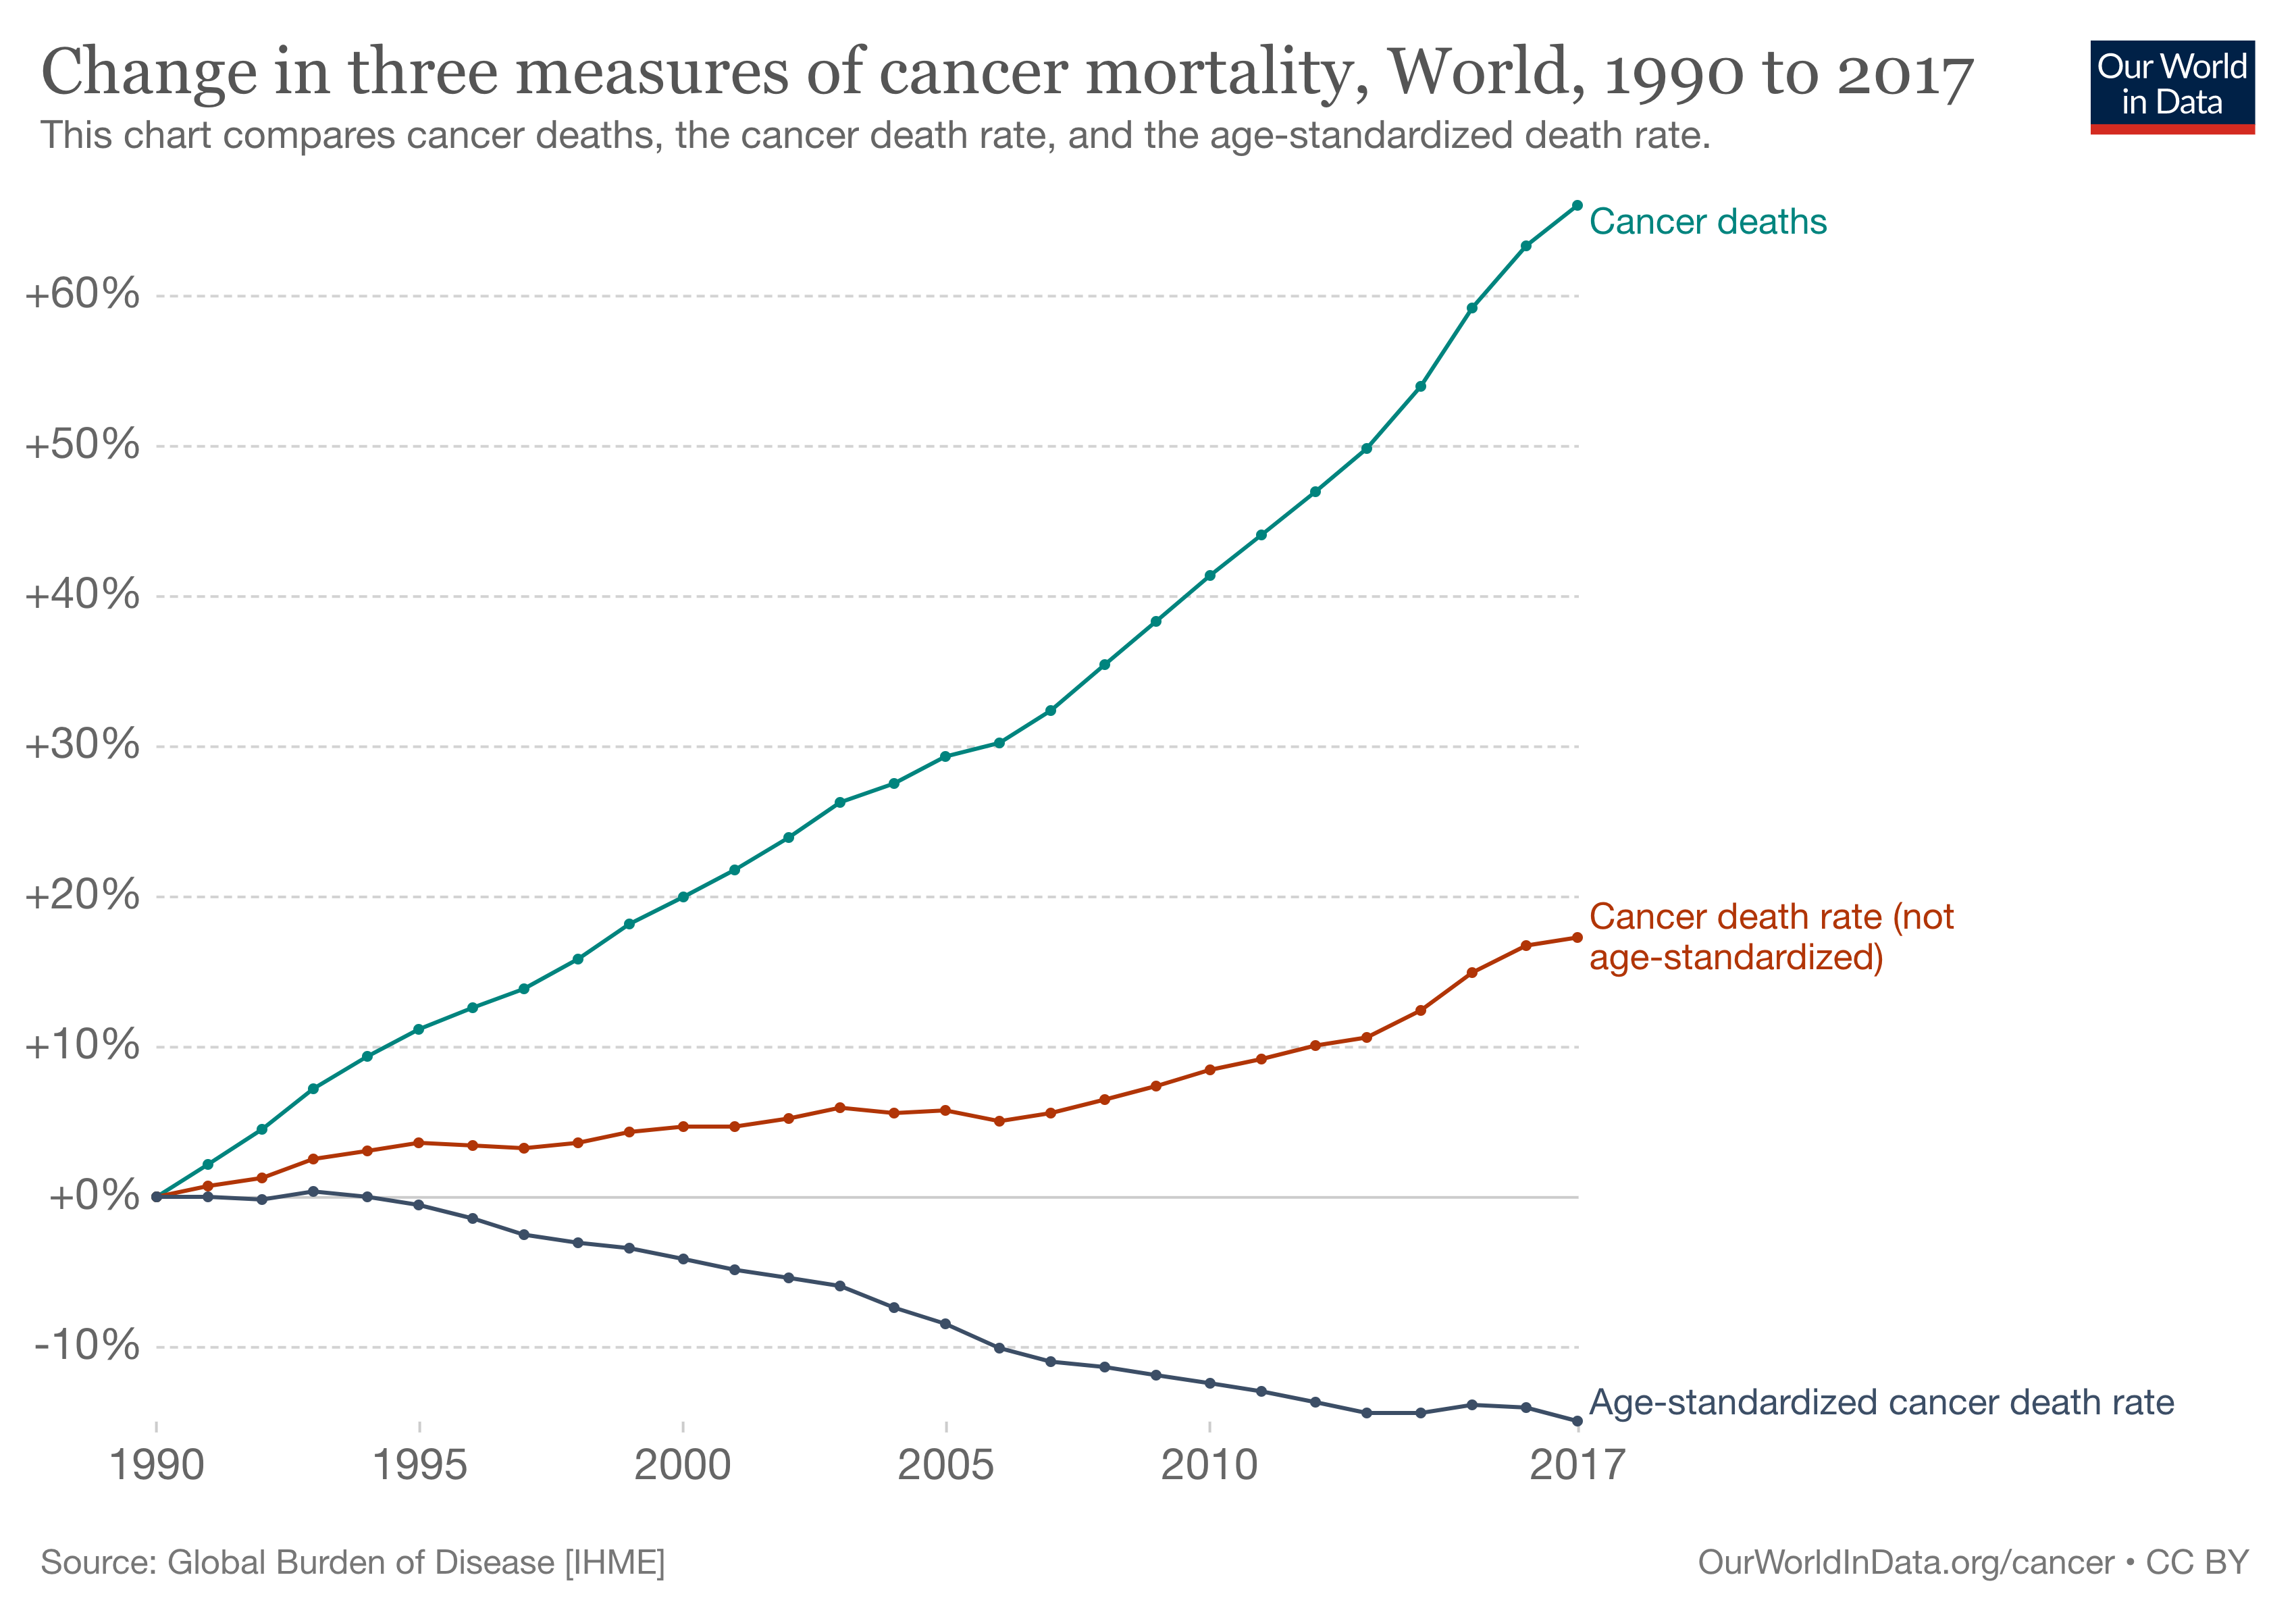
\includegraphics[width=1.0\textwidth,keepaspectratio]{Images/cancer-deaths-rate-and-age-standardized-rate-index.png}
      \caption{Changes in cancer mortality between 1990 and 2017. \citep{Roser2015-qb}}
      \label{fig:cancer_death}
\end{figure}


\section{Aims}

The project's hypothesis proposes that integrating additional data types into the gene expression data will result in MIBC subtypes that more accurately represent the molecular biology of the samples. Especially by combining the gene expression of the non-tumour samples with the mutations and expressed genes in the tumour, it will lead to new MIBC subgroups. Based on this, the project aims can be defined as follows:

\begin{enumerate}
    \item Create a method that allows the integration of multiple data types
    \item Utilise non-cancerous gene expression to inform tumour classifications
    \item Enable researchers to trace the biological mechanisms behind each subtype
\end{enumerate}

While working on achieving the research aims stated above, the research was guided by the following principles:

\begin{itemize}
    \item Data representation needs to be a close approximation of the biology
    \item Traceability - allows the researchers to understand and explain the outputs of the approach used
    \item Ensure the method is modular and data-agnostic, allowing its application to other diseases
    \item Keep the software or the method simple; the complexity arises from the biology
    \item Develop a platform that enables the integration of additional data types beyond those considered in this PhD project
\end{itemize}

% Thesis outline
\section{Thesis Outline}

\textbf{Background} - This chapter introduces the reader to the current state of research on MIBC and the various classification systems found in the literature. It continues by presenting the datasets and methods used in the project, followed by a review of disease stratification methods beyond bladder cancer and gene expression. The final two sections of the chapter cover network methods used in biological applications and community detection methods for identifying subgroups within a network.


\textbf{Cluster Analysis} - This thesis section delves deeper into the clustering methods used throughout the project, whether to group gene expression data or network outputs. Through a standard clustering analysis process, we discovered that one of the major MIBC groups, the basal subtype, can be further divided into three subgroups with differing immune responses and survival prognoses. Notably, the subgroup with the lowest immune response has the poorest 5-year survival rate.

\textbf{A Network Pipeline for Subtyping} - This research investigates the integration of data into a network approach at three key stages: 1) modelling edge weights proportional to the genes' mutation burden, 2) selective edge pruning, which allows \acrlong{tf} to have more connections than other genes, and 3) using gene expression from freshly isolated samples to build a network representation. The chapter assesses the impact of these data integration strategies on the network's metrics.


\textbf{Selective Edge Pruning} - This chapter extends the previous work focusing on finding the appropriate configuration for the number of edges assigned to TF genes and comparing the Leiden community detection algorithm with \acrfull{sbm}. From the selective edge pruning experiments, 98 TFs were identified as naturally co-expressed with other genes, even in a control network. Using the tumour gene expression of this subset to stratify the TCGA's MIBC cohort, a Basal subgroup of 30 samples was discovered, characterised by the lowest survival prognosis in the literature. Notably, this subgroup does not contain samples previously classified as \acrlong{ne} and exhibits squamous phenotypes. \acrshort{sbm} is preferred for community detection as it identifies more communities and is robust in detecting patterns in random data.


\textbf{Network II} - Building on the previous work, this chapter introduces a more refined network approach where the data integration methods from Chapter 4 are adapted to have a larger impact on the network. The research presented identifies 122 genes (TF and non-TF) concentrated in small communities (\(<10\) nodes) that are highly and strongly correlated, as well as having a high mutation burden. This suggests that the network approach can handle larger network sizes. The analysis showed that many of the significantly differentially expressed genes are identified by Ensembl IDs, highlighting the limits of current biological knowledge.


\textbf{Discussion \& Future Work} - This chapter presents the significance and implications of the findings throughout the project and discusses potential avenues for future research.


% Contribution to knowledge
\section{Contributions of each chapter}

\subsection*{Cluster analysis}

\begin{itemize}
    \item Three basal subgroups with heterogenous \acrfull{ifn} immune response
    \item The basal group with the lowest immune response exhibits the worst 5-year survival rate
    \item The basal samples with a strong \acrshort{ifn} response show a more favourable prognosis and can represent potential treatment targets
    \item An aggressive gene filtering of the expressed genes contributes to the findings of the new Basal groups
\end{itemize}

\subsection*{Network I}

\begin{itemize}
    \item Validates the network approach as an integrative method for MIBC stratification
     \item Integration of the mutation burden and TFs affect the network, community detection and MIBC stratifications
     \item Network generated from the gene expression obtained from freshly isolated cells finds different groups from the tumour network representation
\end{itemize}

\subsection*{Selective Edge pruning}

\begin{itemize}
    \item Selective edge pruning as a method to find highly correlated genes in gene expression datasets 
    \item 98 TFs drive a three-way basal split
    \item The Basal group of 20 samples exhibiting squamous markers has the lowest survival prognosis seen in the project and possibly in the literature
    \item Compares two classes of community detection methods in the biological networks
\end{itemize}

\subsection*{Network II}

This chapter brings the following contributions to the field:
\begin{itemize}
    \item A more advanced network pipeline is used to form a non-tumour network representation from which the \acrshort{mibc} is informed
    \item Identification of a subset of genes and communities with a high mutation burden, which are highly and strongly co-expressed with other genes
    \item \acrfull{hsbm} from the network pipeline finds small communities off less than 10 genes in a network of 5000 nodes
    \item Discovery of new Basal and Luminal subdivisions: the former has a low survival rate, and the latter has the highest survival rate over five years. Both are characterised by communities with Ensembl genes,
    \item Identifying new splits in the Abs-Ca and P0 datasets which are enriched by some of the same communities with Ensembl genes from previous point 
    \item An explainable computational solution which allows tracing the result (i.e. subtyping) to network communities and implicitly to a subset of genes
    \item Across the analysis, many differentially expressed genes were found to be Ensembl genes, highlighting the potential for discovering new biological insights
    \item Development of a Python package that gene the network, which is planned to be released to the research community
\end{itemize}